\documentclass[../appunti-analisi.tex]{subfiles}

\begin{document}

\section{Lezione 13}

\textbf{Risoluzione esercizio}

\[
    z = x^{2}+9y^{2}
\]

Il dominio:

\[
    E_k= \{(x,y) \in \mathbb{R}^{2};x^{2}+9y^{2}=k\}
\]

se $k=0$:

\[
    E_0=(0,0)\text{ origine}
\]

se $k>0$ allora otteniamo delle ellissi:

\[
    \frac{x^{2}}{a^{2}}+ \frac{y^{2}}{ \frac{k}{9}} = 1
\]

\textbf{Altro esercizio} 

\[
    z= \frac{y}{x^{2}}
\]

dominio

\[
    E_k = \{(x,y) \in \mathbb{R}^{2};x+2y=k\}
\]

\[
    y=-\frac{1}{2} + \frac{x}{2}
\]


Fascio di rette parallele a $y = -\frac{1}{2}x$

% \begin{figure}[ht]
%     \centering
%     \incfig{fascio-di-rette-parallelo}
%     \caption{fascio di rette parallelo}
%     \label{fig:fascio-di-rette-parallelo}
% \end{figure}

\textbf{Altro esercizio} 

\[
    z= \underbrace{\frac{y}{x^{2}}}_{f(x,y)}
\]

dominio: 

\[
    E_k = \{(x,y) \in \mathbb{R}^{2}; x \neq  0; \frac{y}{x^{2}}=k\}
\]

se $k=0$, è $E_0$ privata dell'origine:

\[
    \frac{y}{x^{2}}=0
\]

se $k>0$:

\[
    \frac{y}{x^{2}} = k
\]

\[
    y = kx^{2}
\]

quindi sono parabole con concavità verso l'alto.

\begin{center}
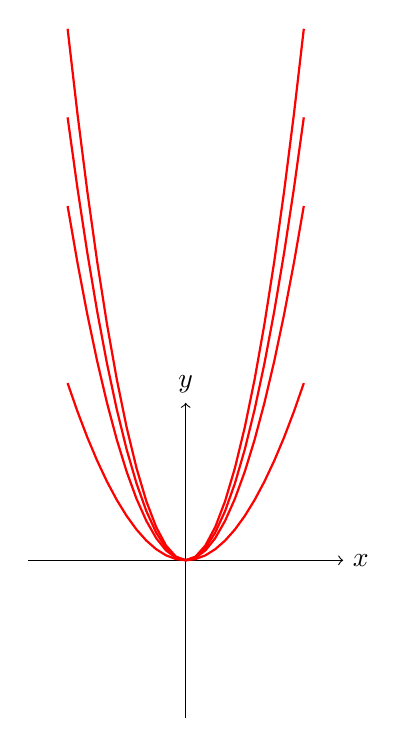
\begin{tikzpicture}
    \draw[->] (-2,0) -- (2,0) node[right] {$x$}; % assi %coordinate
    \draw[->] (0,-2) -- (0,2) node[above] {$y$};
    %parabole y/x^2=k
    \foreach \k in {1,2,3,2.5} {
        \draw[red, thick] plot[domain=-1.5:1.5] (\x, {\k*(\x)^2});
    }
\end{tikzpicture}
\end{center}


se $k<0$ avranno concavità verso il basso

\begin{center}
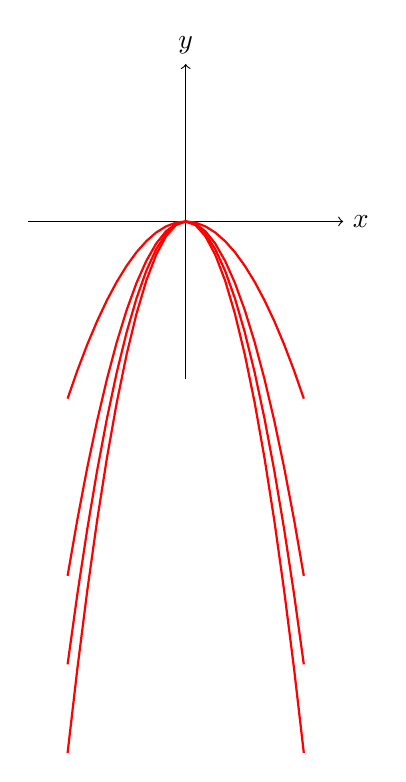
\begin{tikzpicture}
    \draw[->] (-2,0) -- (2,0) node[right] {$x$}; % assi %coordinate
    \draw[->] (0,-2) -- (0,2) node[above] {$y$};
    %parabole y/x^2=k
    \foreach \k in {-1,-2,-3,-2.5} {
        \draw[red, thick] plot[domain=-1.5:1.5] (\x, {\k*(\x)^2});
    }
\end{tikzpicture}
\end{center}


\newpage

\textbf{Esempio limiti} 

\[
    \lim_{ (x,y) \to (0,0) } \frac{xy(2y^{2}+x^{3})}{x^{4}+y^{2}}
\]

Consideriamo le restrizione della funzione lungo le rette $y=mx$:


\[
    \underbrace{\lim_{ (x,y) \to (0,0) }}_{y=mx} f(x,y) = \underbrace{\lim_{ (x,y) \to (0,0) }}_{y=mx} \frac{xmx(2m^{2}x^{2}+x^{3})}{x^{4}+m^{2}x^{2}}= \lim_{ x \to 0 } \frac{mx^{2}(2m^{2}+x)}{(x^{2}+m^{2})} = 0
\]

il limite quindi se esiste deve essere zero. Passiamo adesso alle coordinate polari per valutare $f$:

\[
    |f(\rho, \theta)| = | \frac{\rho cos \theta \rho sin \theta (2 \rho^{2}sin^{2}\theta+\rho^{3}cos^{3}\theta)}{\rho^{4}cos^{4}\theta+\rho^{2}sin^{2}\theta}| = |\frac{\rho^{2}cos \theta sin \theta(2sin^{2}\theta+\rho cos^{2}\theta}{\rho^{2}cos^{4}\theta+sin^{2}\theta}|
\]

quindi:

\[
    |f(\rho, \theta)| = |\frac{2 \rho^{2}cos \theta sin^{3}\theta}{\rho^{2}cos^{4}\theta+sin^{2}\theta}+ \frac{\rho^{3}cos^{4}\theta sin \theta}{\rho^{2} cos^{4}\theta + sin^{2}\theta}| \le |\frac{\rho^{2}cos \theta sin^{3}\theta}{\rho^{2}cos^{4}\theta+sin^{2}\theta}| + |\frac{\rho^{3}cos^{4}\theta sin \theta}{\rho^{2} cos^{4}\theta + sin^{2}\theta}|
\]

\[
    |f(\rho, \theta)| \le \frac{2 \rho^{2} |cos \theta sin^{3} \theta|}{\underbrace{\rho^{2}cos^{4}\theta+sin^{2}\theta}_{\ge 0}} + \frac{\rho^{3}cos^{4}\theta|sin \theta|}{\rho^{2}cos^{4}\theta+\underbrace{sin^{2}\theta}_{\ge 0}} \le \frac{2 \rho^{2}|cos \theta sin^{3}\theta|}{sin^{2}\theta} = 2 \rho^{2} |cos \theta sin \theta| + \rho | sin \theta|
\]

infine quindi (data la limitatezza del $sin$ e del $cos$):

\[
 |f(\rho, \theta)| \le 2 \rho^{2} | cos \theta sin \theta| + \rho|sin \theta| \le 2 \rho^{2} + \rho \underbrace{\rightarrow}_{p \rightarrow 0^{+}} 0
\]


Potevamo però usare un altro metodo senza coordinate polari:

\[
    |f(x,y)|=  |\frac{xy(2y^{2}+x^{3})}{x^{4}+y^{2}}| = |\frac{2xy^{3}+x^{4}y}{x^{4}+y^{2}}| = | \frac{2xy^{3}}{x^{4}+y^{2}}+ \frac{x^{4}y}{x^{4}+y^{2}}| \le |\frac{2xy^{3}}{x^{4}+y^{2}}|+ |\frac{x^{4}y}{x^{4}+y^{2}}|
\]

quindi:

\[
   |f(x,y)|  \le \frac{2|xy^{3}|}{x^{4}+y^{2}} + \frac{x^{4}|y|}{x^{4}+y^{2}} \le \frac{2|xy^{3}|}{y^{2}} + \frac{x^{4}|y|}{x^{4}}
\]

\[
   |f(x,y)|  \le \underbrace{2 |xy| + |y|}_{g(x,y)}
\]

e quindi il limite di $g(x,y)$ (dato che la funzione è continua):

\[
    \lim_{ (x,y) \to (0,0) } g(x,y) = g(0,0) = 0
\]


\textbf{Esercizio limite 2} 

\[
    \lim_{ (x,y) \to (0,0) } \frac{x sin^{2}y+ 3xy^{4}}{x^{2}+2y^{4}}  
\]

riscrivo la $f$ come somma di due funzioni:

\[
    f(x,y) = \frac{x sin^{2}y+ 3xy^{4}}{x^{2}+2y^{4}}  = \underbrace{\frac{x sin^{2}y}{x^{2}+2y^{4}}}_{f_1(x,y)} + \underbrace{\frac{3xy^{4}}{x^{2}+2y^{4}}}_{f_2(x,y)}
\]

\[
    |f_2(x,y)| = | \frac{3xy^{4}}{x^{2}+2y^{4}}| =\frac{3y^{4}|x|}{x^{2}+2y^{4}} \le \frac{3y^{4}|x|}{2y^{4}} \rightarrow 0
\]

vediamo la prima funzione:

\[
    f_1(x,y) = \frac{xsin^{2}y}{x^{2}+2y^{4}}
\]

il numeratore di questa, se trasformiamo in coordinate polari, è come $\rho^{3}$, controllo quindi il denominatore:

\[
    x^{2} + 2y^{4}
\]

il limite potrebbe non esistere, controlliamolo. Per $y=x$:

\[
    \underbrace{\lim_{ (x,y) \to (0,0) }}_{y=x} f_1(x,y) = \lim_{ x \to 0 } \frac{x sin^{2}x}{x^{2}+2x^{4}} = \lim_{ x \to 0 } \frac{x sin^{2}x}{x^{2}(1+2x^{2})} = 0
\]

Per $x = y^{2}$:

\[
    \underbrace{\lim_{ (x,y) \to (0,0) }}_{x=y^{2}} f_1(x,y)  = \lim_{ y \to 0 } \frac{y^{2}sin^{2}y}{y^{4}+2y^{4}} = \lim_{ y \to 0 } \frac{y^{2}sin^{2}y}{3y^{2}}  = \frac{1}{3}
\]

quindi il limite non esiste perché $f= f_1+f_2$ e $\lim_{ (x,y) \to (0,0) } f_2=0$ e $\lim_{ (x,y) \to (0,0) } f_1$ non esiste.

\subsection{Scelta delle curve di restrizione}

Nell'esercizio di prima come ho fatto a restringere la $f_1$?

Vediamolo:

\begin{itemize}
    \item $y=x$ peso le variabili allo stesso modo e dunque il denominatore ($x^{2}+2y^{4}$) ottengo $x^{2}+2x^{4}$ voglio capire che succede per $x \rightarrow 0$.
    \item $x=y^{2}$ il denominatore ($x^{2}+2y^{4}$) ottengo $y^{4}+2y^{4} = 3y^{4}$ quindi qua non trascurare gli addendi.
\end{itemize}

\textbf{Esempio}:

\[
    x^{6} + 3y^{4}
\]

quindi $x=y$ e poi $y = x^{ \frac{2}{3}}$

\textbf{Altro esempio} 

\[
\lim_{ (x,y) \to (0,0) } ( \frac{xy^{2}+2y^{ \frac{1}{3}}sin^{2}x}{x^{2}+y^{2}}) e ^{ \frac{x^{2}-y^{2}}{x^{2}+y^{2}}}
\]

l'esponente non ha limite però:

\[
    0< e ^{ \frac{x^{2}-y^{2}}{x^{2}+y^{2}}} 
\]

vediamo l'esponente:

\[
    \frac{x^{2}-y^{2}}{x^{2}+y^{2}} \le |\frac{x^{2}-y^{2}}{x^{2}+y^{2}}| = \frac{|x^{2}-y^{2}|}{x^{2}+y^{2}}  \le \frac{|x^{2}|+|y^{2}|}{x^{2}+y^{2}} = \frac{x^{2}+y^{2}}{x^{2}+y^{2}} = 1
\]

quindi l'esponenziale è:

\[
    0< e ^{ \frac{x^{2}-y^{2}}{x^{2}+y^{2}}} < e
\]


ora studiamo l'altra parte della funzione $f(x,y)$ in coordinate polari:

\[
    | \frac{\rho cos \theta \rho^{2}sin^{2}\theta + 2 \rho^{ \frac{1}{3}}(sin \theta)^{ \frac{1}{3}}sin^{2}(\rho cos \theta)}{\rho^{2}}| \le  | \frac{\rho^{3}cos \theta sin^{2}\theta}{\rho^{2}}| + |\frac{2 \rho^{ \frac{1}{3}}\rho^{2}cos^{2}\theta (sin \theta)^{ \frac{1}{3}}}{\rho^{2}}| \le 
\]

\[
    \le | \rho cos \theta sin ^{2}\theta| + 2 \rho^{ \frac{1}{3}} | cos^{2}\theta| \le \rho + 2 \rho^{ \frac{1}{3}} \rightarrow 0
\]

quindi alla fine il limite:

\[
    \lim_{ (x,y) \to (0,0) } f(x,y)=0
\]

\end{document}
